\setchapterimage[6cm]{chapter/country/Political_Map_of_the_World_2013.jpg}
%\setchapterstyle{kao}
\setchapterpreamble[u]{\margintoc}
\chapter{Analysis of aspects of modern countries\protect\footnotemark}
\labch{country}

\footnotetext{\href{https://en.wikipedia.org/wiki/World_map}{Political map of the world}. 
	Author: \href{https://commons.wikimedia.org/wiki/File:Political_Map_of_the_World,_2013.png}{Central Intelligence Agency / 2015 /  Creative Commons Attribution License}.}

The chapter is devoted to the study of countries based on the knowledge base of the Wikidata international project. SPARQL queries were used in order to analyse and compare ``countries'' objects in Wikidata. A list of all currently existing countries, a list of countries ordered by date of creation, a list of demonyms of countries were generated. A bubble chart with the forms of government of countries, a graph of neighboring countries and a map of neighboring countries of Russia were constructed. In addition, conclusions were drawn regarding the completeness of the Wikidata for this topic.

%%%%%%%%%%%%%%%%%%%%%%%%%%%%%%%%%%%%%%%%%%%%%%%%%%%%%%%
\section{Instances}

Let's build a list of all countries in English and Russian (Listing \ref{lst:country}).

\begin{lstlisting}[ language=SPARQL, 
caption={List of countries in English and Russian. The result contains \num{205} countries in 2017 and \num{175} in 2020.\\\hspace{\textwidth}
SPARQL query: \href{https://w.wiki/k6L}{https://w.wiki/k6L}
},
label=lst:country]
#List of countries in English and Russian
SELECT ?country ?label_en ?label_ru
WHERE
{
	?country wdt:P31 wd:Q6256. # instance country
	?country rdfs:label ?label_en filter (lang(?label_en) = "en").
	?country rdfs:label ?label_ru filter (lang(?label_ru) = "ru").
}
\end{lstlisting}


\begin{marginfigure}[0.0cm]
	{
		\setlength{\fboxsep}{0pt}%
		\setlength{\fboxrule}{1pt}%
		\fcolorbox{gray}{gray}{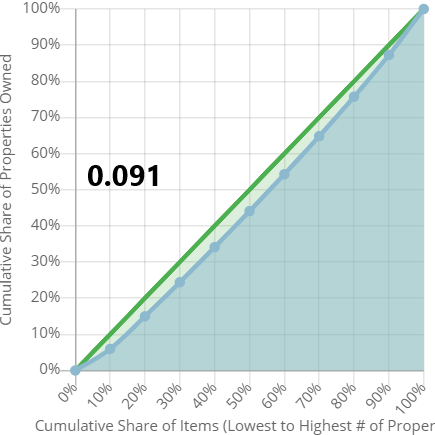
\includegraphics{chapter/country/ProWD_country.png}}
	}
    \caption[Number of properties of instances of the Wikidata object Country.]{%
		High degree of filling according to the number of properties of the Wikidata object \href{https://www.wikidata.org/wiki/Q6256}{Country (Q6256)}.  
		Data obtained using the service \href{https://prowd.id/dashboards/86b6f91a8131/profile}{ProWD.id}, 2020. \emph{The Gini coefficient is 0.091.}
	}%
	\label{fig:ProWD_country}%
\end{marginfigure}

According to the degree of occupancy of properties on Wikidann, one can distinguish between ``full'' and ``empty'' countries.

Examples of the most complete and developed countries on Wikidata according to ProWD\sidecite{prowd_balakireva} are: \wdqName{Israel}{801}, \wdqName{France}{142}, \wdqName{United States of America}{30}. According to ProWD, the leaders among the countries in terms of the number of properties in Wikidata are \wdqName{Israel}{801} and \wdqName{France}{142} (127 properties each), the lowest number of properties is in the \wdqName{Democratic Republic of Vietnam}{172640}  (24 properties).


%%%%%%%%%%%%%%%%%%%%%%%%%%%%%%%%%%%%%%%%%%%%%%%%%%%%%%%
\section{Age of countries and why Russia is not a country? About p:/ps: construction}
\labsec{RussiaNotCountryPPS}

Let's build a list of countries sorted by the date of the country's foundation (the first mention of the country) (Listing \ref{lst:age_of_country}).

\begin{lstlisting}[ language=SPARQL, 
caption={List of countries sorted by inception date. The result contains \num{112} countries with date of inception (foundation) in 2017 and \num{187} in 2021. But this list of countries do not contain, for example, Russia. \\\hspace{\textwidth}
SPARQL query: \href{https://w.wiki/vJk}{https://w.wiki/vJk}
},
label=lst:age_of_country, 					
]
# List of countries sorted by inception 
SELECT ?country ?countryLabel ?inception
WHERE
{
	?country wdt:P31 wd:Q6256.    # instance of country
	?country wdt:P571 ?inception. # the first mention
	SERVICE wikibase:label { bd:serviceParam wikibase:language "en" }
}
ORDER BY (?inception)
\end{lstlisting}

As a result of executing the request (listing \ref{lst:age_of_country}), a modest list of countries was obtained, including only 184 countries for 2020. Using the example of Russia, we will figure out what is the matter here. The \wdqName{Russia}{159} object in the ``instance of'' field contains not one, but eight values, including \wdqName{country}{6256}.

\marginnote{%
    On the Wikidata page ``Request a query'' some editors ask questions about writing scripts, while other editors answer. Use this forum: \href{https://w.wiki/tLm}{https://w.wiki/tLm}.
}
The solution and the answer to this question were found on the page ``Wikidata: Request a query'', namely in the section available at the link \href{https://w.wiki/tLm}{https://w.wiki/tLm}.

The point is that the \emph{wdt} construction allows you to find only true values. 
For Russia, the preferred value in the ``instance of'' field is a sovereign state, not a country. 
To check all the options presented in the ``instance of'' field in Russia, 
you need to use the \emph{p:/ps:} construction.

Thus, the script for getting all 232 countries sorted by creation date is shown in the listing~\ref{lst:list_of_country_instance_of}.

\begin{lstlisting}[ language=SPARQL, 
caption={List of countries sorted by inception date. The result contains \num{112} countries with completed date of foundation in 2017 and \num{235} in 2021.\\\hspace{\textwidth}
SPARQL query: \href{https://w.wiki/vJp}{https://w.wiki/vJp}
},
label=lst:list_of_country_instance_of, 					
]
# List of countries sorted by inception date
SELECT ?country ?countryLabel
(MIN(?year) AS ?min_year)
WHERE
{
	?country p:P31 [ps:P31 wd:Q6256]. # instance of a country 
	?country p:P571 [ps:P571 ?inception]. # all inception dates
	BIND(YEAR(?inception) AS ?year)
	SERVICE wikibase:label { bd:serviceParam wikibase:language "en" }
}
GROUP BY ?country ?countryLabel ?min_year
ORDER BY ?min_year
\end{lstlisting}

To remove from this list no longer existing countries, that is, instances of the \wdqName{historical country}{3024240} object, use the MIN US operator.

Using the script (listing \ref{lst:list_of_country_instance_of_}), 211 non-historical countries with a known foundation date were obtained.
\index{SPARQL!MINUS!List of countries sorted by inception date}
\begin{lstlisting}[ language=SPARQL, 
caption={List of countries sorted by inception date. The result contains \num{112} countries with completed date of foundation in 2017 and \num{211} in 2021.\\\hspace{\textwidth}
SPARQL query: \href{https://w.wiki/vJt}{https://w.wiki/vJt}
},
label=lst:list_of_country_instance_of_, 					
]
# List of countries sorted by inception date
SELECT ?country ?countryLabel 
(MIN(?year) AS ?min_year)
WHERE
{
	?country p:P31 [ps:P31 wd:Q6256]. # instance of a country 
	MINUS {?country p:P31 [ps:P31 wd:Q3024240]}. # except historical countries
	?country p:P571 [ps:P571 ?inception]. # all inception dates
	BIND(YEAR(?inception) AS ?year)
	SERVICE wikibase:label { bd:serviceParam wikibase:language "en" }
}
GROUP BY ?country ?countryLabel ?min_year
ORDER BY ?min_year
\end{lstlisting}


For example, \wdqName{France}{142}~--- 463 year, \wdqName{Russia}{159}~--- 862, \wdqName{Republic of Kosovo}{1246}~--- 2008, \wdqName{South Sudan }{958}~--- 2011.
The largest number of countries appeared in 1960 (16 countries), in 1991 (15 countries), in 1962 (6 countries) and in 1821 (6 countries).

Let's display a list of countries with an empty ``inception of'' property (Listing \ref{lst:without_inception}).
\index{SPARQL!MINUS!List of countries without a inception}
\begin{lstlisting}[ language=SPARQL, 
caption={List of `instances of` ``countries without a inception''. The result contains \num{100} countries without completed date of foundation in 2017 and \num{7} in 2020.\\\hspace{\textwidth}
SPARQL query: \href{https://w.wiki/k6q}{https://w.wiki/k6q}},
label=lst:without_inception
]
SELECT ?country ?countryLabel 
WHERE
{
	?country wdt:P31 wd:Q6256. # country
	MINUS { ?country wdt:P571 [] }. # inception of country is empty
	SERVICE wikibase:label { bd:serviceParam wikibase:language "en" }
}
\end{lstlisting}

%So, on March 6 2017, the Wikidata contains 100 out of 198 entries about the currently existing countries with an unknown year of the country's foundation.

%%%%%%%%%%%%%%%% Ex 3 %%%%%%%%%%%%%%%%
\marginnote[-2.0cm]{
	\label{question:population_density}
	Identify the countries of Asia by flags and list them in ascending order of population density (fig. ~\ref{fig:flag_kor}, ~\ref{fig:flag_mongolia}, ~\ref{fig:flag_singapore}, ~\ref{fig:flag_israel}).
}

\begin{marginfigure}[0.0cm]
	{
		\setlength{\fboxsep}{0pt}%
		\setlength{\fboxrule}{1pt}%
		\fcolorbox{gray}{gray}{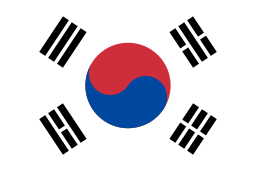
\includegraphics[width=\linewidth]{./chapter/country/256px-Flag_of_South_Korea.png}}%
	}
	\caption{First country flag.}%
	\label{fig:flag_kor}%
\end{marginfigure}

\begin{marginfigure}[4.0cm]
	{
		\setlength{\fboxsep}{0pt}%
		\setlength{\fboxrule}{1pt}%
		\fcolorbox{gray}{gray}{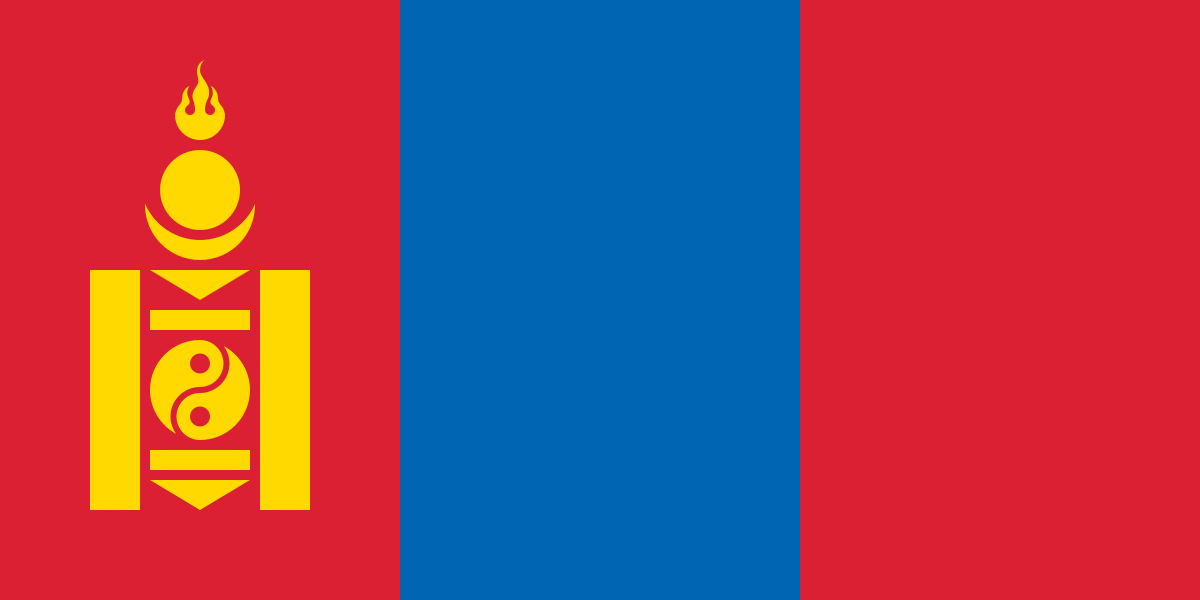
\includegraphics[width=\linewidth]{./chapter/country/256px-Flag_of_Mongolia.png}}%
	}
	\caption{Second country flag.}%
	\label{fig:flag_mongolia}%
\end{marginfigure}


\subsection{Completeness of Wikidata}

Let's analyze the completeness of Wikidata: historical and modern countries.

According to the ``Russian classification of countries of the world''\sidecite{oksm} there are 251 countries on earth.

This task does not take into account ancient, non-existent states (for example: \wdqName{Assyria}{41137}), since they are not a ``country'' object but a ``historical country'' object. Let us note that the number of historical countries is an order of magnitude greater than the existing countries.


Using the script (Listing \ref{lst:List_of_historical_countries}), let's build a list of historical states. There were three thousand such former states, which is an order of magnitude more than the number of modern states.

\begin{lstlisting}[ language=SPARQL, 
caption={List of historical countries. The result contains \num{3025} countries without completed date of foundation in 2021.\\\hspace{\textwidth}
SPARQL query: \href{https://w.wiki/vRV}{https://w.wiki/vRV}},
label=lst:without_inception
]
# List of historical countries
SELECT ?country ?countryLabel
WHERE
{
	?country p:P31 [ps:P31 wd:Q3024240]. # instance of a historical country 
	SERVICE wikibase:label { bd:serviceParam wikibase:language "[AUTO_LANGUAGE],en,ru"} 
}
\end{lstlisting}

\marginnote{
	\label{question:old_countries}
	Find the states that have existed the longest.
}

\marginnote{
	See the answer in Exercise~\ref{answer:old_countries}, page~\pageref{answer:old_countries}.
}

According to the category of \href{https://w.wiki/dWv}{``Alphabetical list of countries and territories''}\sidecite{list_of_sovereign_states} in Russian Wikipedia, there are 252 countries.

According to the category of \href{https://en.wikipedia.org/wiki/List_of_sovereign_states}{``List of sovereign states''}\sidecite{list_of_sovereign_states_en} in English Wikipedia, there are 206 countries.

\begin{marginfigure}[0.0cm]
	{
		\setlength{\fboxsep}{0pt}%
		\setlength{\fboxrule}{1pt}%
		\fcolorbox{gray}{gray}{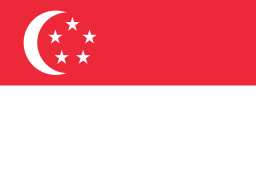
\includegraphics[width=\linewidth]{./chapter/country/256px-Flag_of_Singapore.png}}%
	}
	\caption{Third country flag.}%
	\label{fig:flag_singapore}%
\end{marginfigure}

\begin{marginfigure}[4.0cm]
	{
		\setlength{\fboxsep}{0pt}%
		\setlength{\fboxrule}{1pt}%
		\fcolorbox{gray}{gray}{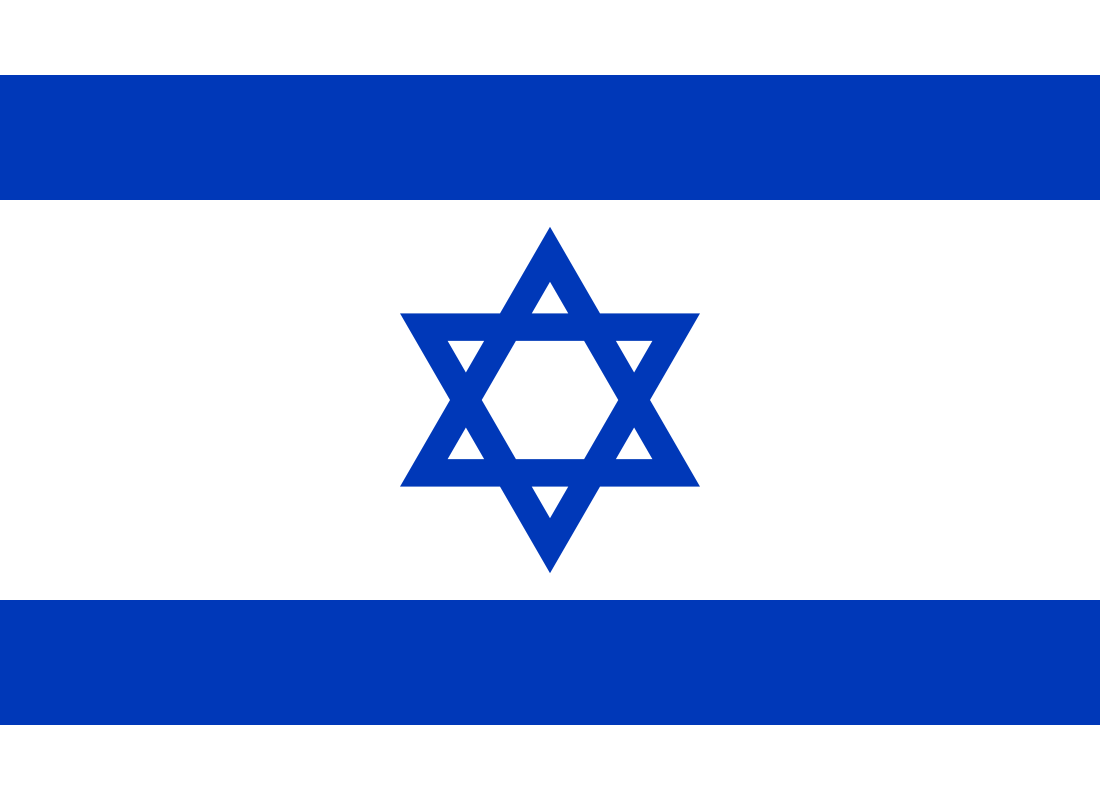
\includegraphics[width=\linewidth]{./chapter/country/256px-Flag_of_Israel.png}}%
	}
	\caption{Fourth country flag.}%
	\label{fig:flag_israel}%
\end{marginfigure}
\marginnote{
	See the answer in Exercise~\ref{answer:population_density}, page~\pageref{answer:population_density}.
}

It is not always possible to specify the exact date of the country's foundation for various reasons: absence, lack or inconsistency of written sources. For example, the basis of the Old Russian state is associated with the vocation of Varangian prince Rurik in 862, but there is no exact date (object \wdqName{Russia}{159}). Also, some modern countries were preceded by a number of others and the date of formation of which of them should be considered as the date of creation of the country is an open question (for example, \wdqName{Mongolia}{711}).


%%%%%%%%%%%%%%%%%%%%%%%%%%%%%%%%%%%%%%%%%%%%%%%%%%%%%%%
\section{List of demonyms in English}

Demonyms~--- is the name of the inhabitants of a certain area, correlated with the toponym. For example, demonyms for Russia will be Russians, a Russian, a Russian woman, for the Czech Republic~--- Czechs.

In addition to the geographical factor, the new lexemes used to determine origin or belonging also come from ethnic, political, religious characteristics of people\sidecite{Zhuravleva2012}.

Demonyms can be defined by the names of different objects of the earth's surface, mountains, islands, continents. Also, the designation of the place of origin of people may depend on the political and administrative division. For example, to denote citizenship: Thailand~--- Thai people, Canada~--- Canadians. Intra-state division can also give rise to new names, Crimea~--- Crimeans.

Let's build a list of countries that have demonyms in English (Listing \ref{lst:demonym}).

\index{SPARQL!FILTER!List of countries with demonyms in English}
\begin{lstlisting}[ language=SPARQL, 
caption={List of countries with demonyms in English. The result contains \num{197} countries with demonyms in 2017 and \num{209} in 2021.\\\hspace{\textwidth}
SPARQL query: \href{https://w.wiki/vRW}{https://w.wiki/vRW}},
label=lst:demonym, 
]
# List of countries with demonyms in English
SELECT ?country ?countryLabel 
WHERE
{
	?country p:P31 [ps:P31 wd:Q6256]. # instance of a country
	?country wdt:P1549 ?demonym .     # has demonym
	FILTER((LANG(?demonym)) = "en")
	SERVICE wikibase:label { bd:serviceParam wikibase:language "en" }
}
GROUP BY ?country ?countryLabel
\end{lstlisting}



\subsection{List of demonyms}

Let's build a list of all demonyms in English (Listing \ref{lst:list_demonym}).

\index{SPARQL!FILTER!List of demonyms in English}
\begin{lstlisting}[ language=SPARQL, 
caption={List of demonyms in English. The result contains \num{237} demonyms in 2017 and \num{296} in 2021.\\\hspace{\textwidth}
SPARQL query: \href{https://w.wiki/vRX}{https://w.wiki/vRX}},
label=lst:list_demonym, 
]
# List of demonyms of countries in English
SELECT ?country ?countryLabel ?demonym
WHERE
{
	?country p:P31 [ps:P31 wd:Q6256]. # instance of a country
	?country wdt:P1549 ?demonym .     # has demonym
	FILTER((LANG(?demonym)) = "en")
	SERVICE wikibase:label { bd:serviceParam wikibase:language "en" }
}
\end{lstlisting}

%SPARQL query (listing ~\ref{lst:list_demonym}), 237 results (2017), 213 results (2020).

%On April 27 2017, the Wikidata contains 237 filled demonyms.

\subsection{Countries with unfilled demonyms}

Let's build a list of countries which do not have demonyms in English (Listing \ref{lst:without_demonym}).
\index{SPARQL!MINUS!List of countries without demonyms in English}
\begin{lstlisting}[ language=SPARQL, 
caption={List of countries without demonyms in English. The result contains \num{5} countries without demonyms in 2017 and \num{9} in 2021.\\\hspace{\textwidth}
SPARQL query: \href{https://w.wiki/myi}{https://w.wiki/myi}},
label=lst:without_demonym, 
]
#List of countries without demonyms in English
SELECT ?country ?countryLabel 
WHERE
{
	?country p:P31 [ps:P31 wd:Q6256].  # instance of a country
	MINUS { ?country wdt:P1549 ?demonym.    # without demonyms
		FILTER((LANG(?demonym)) = "en") # in Russian
	}
	SERVICE wikibase:label { bd:serviceParam wikibase:language "en" }
}
GROUP BY ?country ?countryLabell
\end{lstlisting}

Thanks to the MINUS construction (Listing \ref{lst:without_demonym}), the final list did not include countries with ethno-burial names in Russian.

\subsection{Number of demonyms in countries}

One country can have from zero, if the data is not filled in, to three or four ethnohoronyms. For example, Turkey has three names of its inhabitants: Turks, Tarchanka, Turks, Ethiopia has four: Ethiopian, Ethiopian, Ethiopian, Ethiopian.

Let`s display the list of countries, ordered by the number of demonyms filled in Wikidata (Listing \ref{lst:count_demonym}).

\begin{lstlisting}[ language=SPARQL, 
caption={Count of demonyms in countries. The result contains \num{199} count of demonyms in countries in 2017 and \num{215} in 2021.\\\hspace{\textwidth}
SPARQL query: \href{https://w.wiki/vKD}{https://w.wiki/vKD}},
label=lst:count_demonym, 
]
# List of countries ordered by number of demonyms
SELECT  ?country ?countryLabel (COUNT(*) AS ?demonyms)
WHERE
{
	?country p:P31 [ps:P31 wd:Q6256].# instance of a country
	?country p:P1549 [ps:P1549 []].  # has demonym
	SERVICE wikibase:label {bd:serviceParam wikibase:language "en"}
}
GROUP BY ?country ?countryLabel 
ORDER BY DESC(?demonyms)
\end{lstlisting}

%%%%%%%%%%%%%%%% Ex 4 %%%%%%%%%%%%%%%%
\marginnote{
	\label{question:official_language}
	Which of these languages are official in \href{https://en.wikipedia.org/wiki/Russia}{Russia}?
	\begin{itemize}
		\item \href{https://en.wikipedia.org/wiki/Abaza_language}{Abaza};
		\item \href{https://en.wikipedia.org/wiki/Moksha_language}{Moksha};
		\item \href{https://en.wikipedia.org/wiki/Erzya_language}{Erzya};
		\item \href{https://en.wikipedia.org/wiki/Belarusian_language}{Belarusian}.
	\end{itemize}
}
\marginnote{
	See the answer in Exercise~\ref{answer:official_languages}, page~\pageref{answer:official_languages}.
}

According to data for 2017, the United States of America has the largest number of demonyms (41 demonyms), followed by Great Britain (40), Germany (40) and Canada (36). For 2021, the largest number of demonyms is in Germany (64 demonyms), Russia (61), Canada (60) and the United States (60). Thus, from 2017 to 2021, approximately 20 demonyms were added per country.

%%%%%%%%%%%%%%%%%%%%%%%%%%%%%%%%%%%%%%%%%%%%%%%%%%%%%%%
\section{Basic forms of government}

Let's construct a bubble diagram of countries' government forms (Listing \ref{lst:form_of_government}), where the size of the bubble will correspond to the number of countries with one form of government or another.

\index{SPARQL!FILTER!Forms of government ordered by number of countries}
\index{Chart!BubbleChart!Basic forms of government}
\begin{lstlisting}[ language=SPARQL, 
caption={Basic form of government ranking. The result contains \num{30} basic forms of government in 2017 and \num{41} in 2020.\\\hspace{\textwidth}
SPARQL query: \href{https://w.wiki/vRY}{https://w.wiki/vRY}},
label=lst:form_of_government
]
# Forms of government ordered by number of countries
#defaultView:BubbleChart
SELECT ?bfog ?form (COUNT(*) AS ?countries)
WHERE 
{
	?country p:P31 [ps:P31 wd:Q6256].# instance of a country
	?country p:P122 [ps:P122 ?bfog].# # basic form of government
	OPTIONAL {
	?bfog rdfs:label ?form
		FILTER (LANG(?form) = "en")
	}
	SERVICE wikibase:label { bd:serviceParam wikibase:language "en"}
}
GROUP BY ?bfog ?form
ORDER BY DESC(?countries) ASC(?form)
\end{lstlisting}

%SPARQL query (listing ~\ref{lst:form_of_government}),199 results (2017), 30 results (2017), 29 results (2020).

The variable ``bfog'' (short for ``basic form of government'') contains the form of government, for example, ``republic''.

The last line in Listing \ref{lst:form_of_government} contains the ordering commands first in descending order (DESC) and then ascending order (ASC). Thus, the forms of government are first sorted by the number of countries (?countries). Then, if the countries are equally divided, then the forms of government are sorted lexicographically\protect\footnotemark.

\footnotetext{Lexicographic (dictionary) order~--- is a way of ordering and sorting words, which is commonly used in dictionaries, encyclopedias and alphabetical indexes. For example, A < AA < AAA < AAB < AAC < AB < B < … < ZZZ.}


As a result of the query, we get a bubble chart with the most popular forms of government in countries in 2017 (fig.~\ref{fig:bubble_chart_forms_of_government_countries_2017}) and in 2020 (fig.~\ref{fig:bubble_chart_forms_of_government_countries_2020}).

\begin{figure}
	{
		\setlength{\fboxsep}{0pt}%
		\setlength{\fboxrule}{1pt}%
		\fcolorbox{gray}{gray}{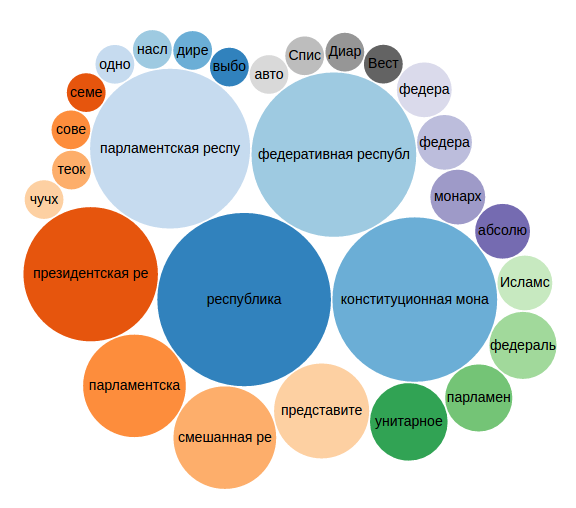
\includegraphics[width=\linewidth]{./chapter/country/Bubble_chart_forms_of_government_countries_according_to_Wikidata.png}}%
	}
	\caption[Bubble chart forms of government countries, 2017]{Bubble chart forms of government countries, 2017
		\\ The popular forms of government of the countries are the republic (in 20 countries), the constitutional monarchy (18), the federal republic (18), the parliamentary republic (17) and the presidential system (11) for 2017.
	}%
	\label{fig:bubble_chart_forms_of_government_countries_2017}%
\end{figure}

\begin{figure}
	{
		\setlength{\fboxsep}{0pt}%
		\setlength{\fboxrule}{1pt}%
		\fcolorbox{gray}{gray}{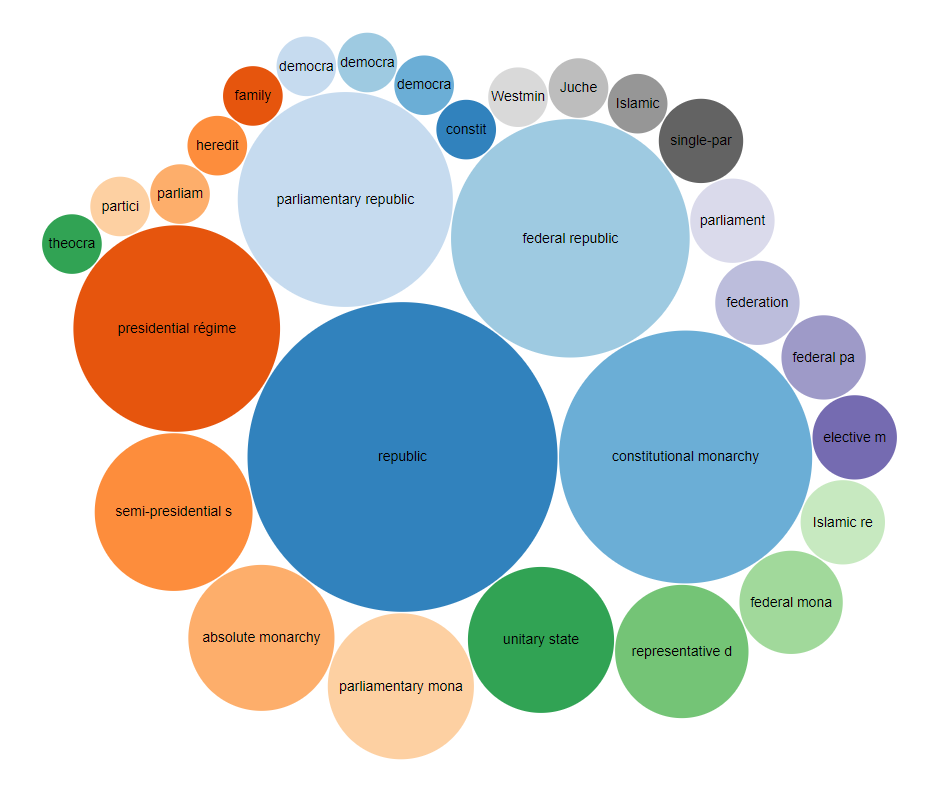
\includegraphics[width=\linewidth]{./chapter/country/Bubble_chart_forms_of_government_countries_according_to_Wikidata_2020.PNG}}%
	}
	\caption
	[Bubble chart forms of government countries, 2020]
	{Bubble chart forms of government countries, 2020
		\\ 
		The popular forms of government of the countries are the republic (in 27 countries), the constitutional monarchy (18), the federal republic (16), the parliamentary republic (13) and the presidential system (12) for 2020.
	}%
	\label{fig:bubble_chart_forms_of_government_countries_2020}%
\end{figure}

Thus, for the period from 2017 to 2020, the form of government ``republic'' became more ``popular''. The number of countries having the form of a ``mixed republic'' has significantly decreased. Forms such as democratic centralism, democratic republic, democracy, Islamic state and parliamentary democracy emerged.

%%%%%%%%%%%%%%%%%%%%%%%%%%%%%%%%%%%%%%%%%%%%%%%%%%%%%%%
\section{Neighboring countries}

Countries have such a property as a common border. On Wikidata, this property is \href{https://www.wikidata.org/wiki/Property:P47}{shares border with (P47)}. Using this property, let's build a graph of neighboring countries (Listing \ref{lst:neighboring_countries}).


\index{Graph!Graph!Neighboring countries}
\begin{lstlisting}[ language=SPARQL, 
caption={Neighboring countries graph. The result contains \num{795} neighboring countries in 2017 and \num{912} in 2020.\\\hspace{\textwidth}
SPARQL query: \href{https://w.wiki/vKR}{https://w.wiki/vKR}},
label=lst:neighboring_countries
]
# Graph of countries which share border
#defaultView:Graph
SELECT ?country ?countryLabel ?border ?borderLabel
WHERE
{
	?country p:P31 [ps:P31 wd:Q6256]. # instance of a country
	OPTIONAL { ?country wdt:P47 ?sharesBorderWith }
	SERVICE wikibase:label {bd:serviceParam wikibase:language "en"}
}
\end{lstlisting}

%SPARQL query (listing ~\ref{lst:neighboring_countries}), 795 results (2017), 698 results (2020).

\begin{figure*}
	{
		\setlength{\fboxsep}{0pt}%
		\setlength{\fboxrule}{1pt}%
		\fcolorbox{gray}{gray}{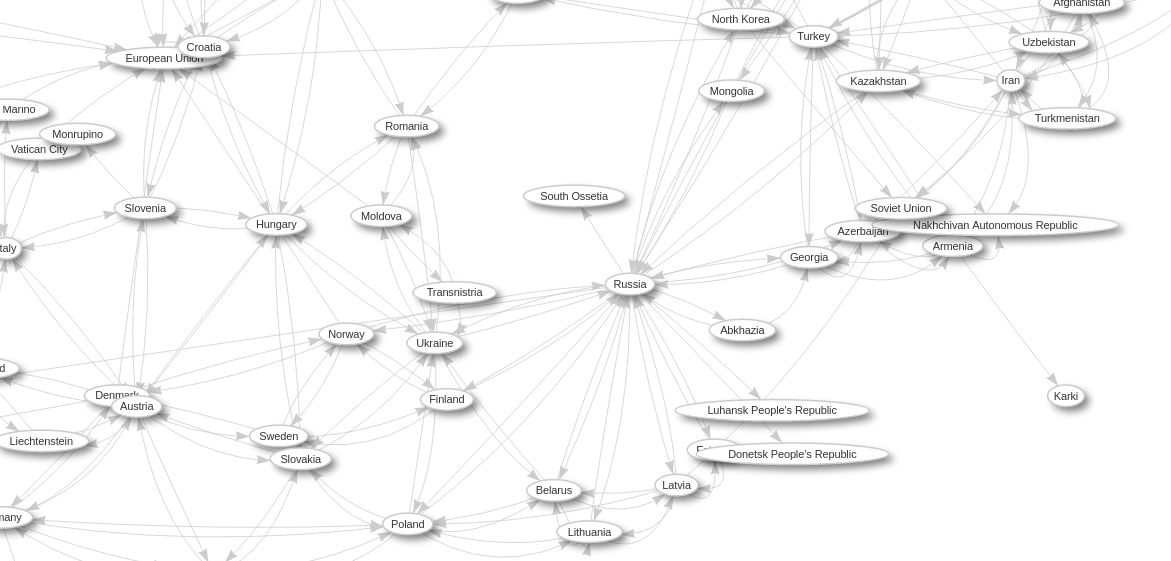
\includegraphics[width=\linewidth]{./chapter/country/Neighboring_countries_graph_according_to_Wikidata.png}}%
	}
	\caption{Neighboring countries graph, 2017.
	}%
	\label{fig:neighboring_countries_2017}%
\end{figure*}

\begin{figure*}
	{
		\setlength{\fboxsep}{0pt}%
		\setlength{\fboxrule}{1pt}%
		\fcolorbox{gray}{gray}{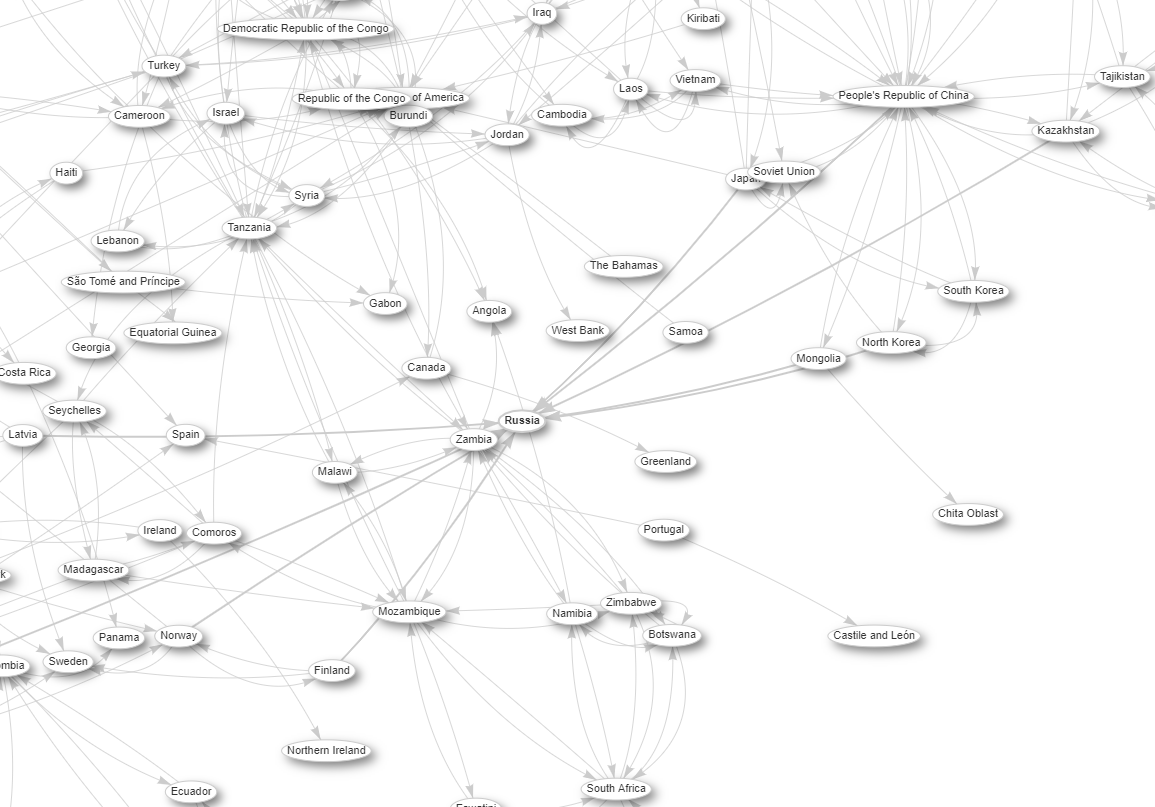
\includegraphics[width=\linewidth]{./chapter/country/Neighboring_countries_graph_in_russian_according_to_Wikidata_2020_en_upload.png}}%
	}
	\caption{Neighboring countries graph, 2020.
	}%
	\label{fig:neighboring_countries_2020}%
\end{figure*}

%%%%%%%%%%%%%%%% Ex 2 %%%%%%%%%%%%%%%%
\marginnote{
	\label{question:administrative_territorial}
	Latvia has 119, Thailand has 77, Denmark has 5, and Russia has 81. What are we talking about?
	\begin{itemize}
		\item Is a number of cities with a population of over one million?
		\item Is a number of higher education institutions?
		\item Is a number of administrative units?
		\item Is a number of official languages?
	\end{itemize}
}

\marginnote{
	See the answer in Exercise~\ref{answer:administrative_territorial}, page~\pageref{answer:administrative_territorial}.
}

As a result of the query, we get a graph with 787 edges on 2017 (fig. ~\ref{fig:neighboring_countries_2017}) and 912 edges on 2020 (fig. ~\ref{fig:neighboring_countries_2020}), where the edge is a neighborhood between the two countries. The graph represents several connected components, since there are island countries that do not have neighbors (for example, Mauritius, Maldives, Madagascar).

\subsection{Neighboring countries of Russia}

We will construct a graph of neighboring countries of Russia (Listing \ref{lst:neighboring_countries_ru}).
\index{Map!Map!Neighboring countries of Russia}
\begin{lstlisting}[ language=SPARQL, 
caption={Map of neighboring countries of Russia. The result contains \num{17} neighboring countries in 2021.\\\hspace{\textwidth}
SPARQL query: \href{https://w.wiki/vKV}{https://w.wiki/vKV}},
label=lst:neighboring_countries_ru
]
# Map of neighboring countries of Russia
#defaultView:Map
SELECT ?border_country ?border_countryLabel ?coords ?layer
WHERE 
{                                         # border_country
	?border_country p:P47 [ps:P47 wd:Q159]. #   has border with Russia
	?border_country p:P31 [ps:P31 wd:Q6256].#   is a country
	OPTIONAL {?border_country wdt:P3896 ?coords.}
	BIND (?coords AS ?layer)
	SERVICE wikibase:label { bd:serviceParam wikibase:language "en". }
}
\end{lstlisting}

The line in Listing \ref{lst:neighboring_countries_ru} with the comment ``is a country'' is needed to check that the object specified as ``having a common border'' with Russia is a country. This made it possible to exclude from the list the region of Georgia (Racha-lechkhumi and Kvemo-Svaneti), and for example, the island of Japan (Hokkaido), indicated in the list of border objects.

As a result of the query execution (Listing \ref{lst:neighboring_countries_ru}), we get a map of neighboring countries of Russia (Fig. ~\ref{fig:neighboring_countries_ru}), including 17 countries, namely: \wdqName{Japan}{17}, \wdqName{Norway}{20}, \wdqName{USA}{30}, \wdqName{Finland}{33}, \wdqName{Sweden}{34}, \wdqName{Poland}{36}, \wdqName{Lithuania}{37}, \wdqName{People's Republic of China}{148}, \wdqName{Belarus}{184}, \wdqName{Estonia}{191}, \wdqName{Latvia}{211}, \wdqName{Ukraine}{212}, \wdqName{Azerbaijan}{227}, \wdqName{Georgia}{230}, \wdqName{Kazakhstan}{232}, \wdqName{DPRK}{423} and \wdqName{Mongolia}{711}.


\begin{figure*}
	{
		\setlength{\fboxsep}{0pt}%
		\setlength{\fboxrule}{1pt}%
		\fcolorbox{gray}{gray}{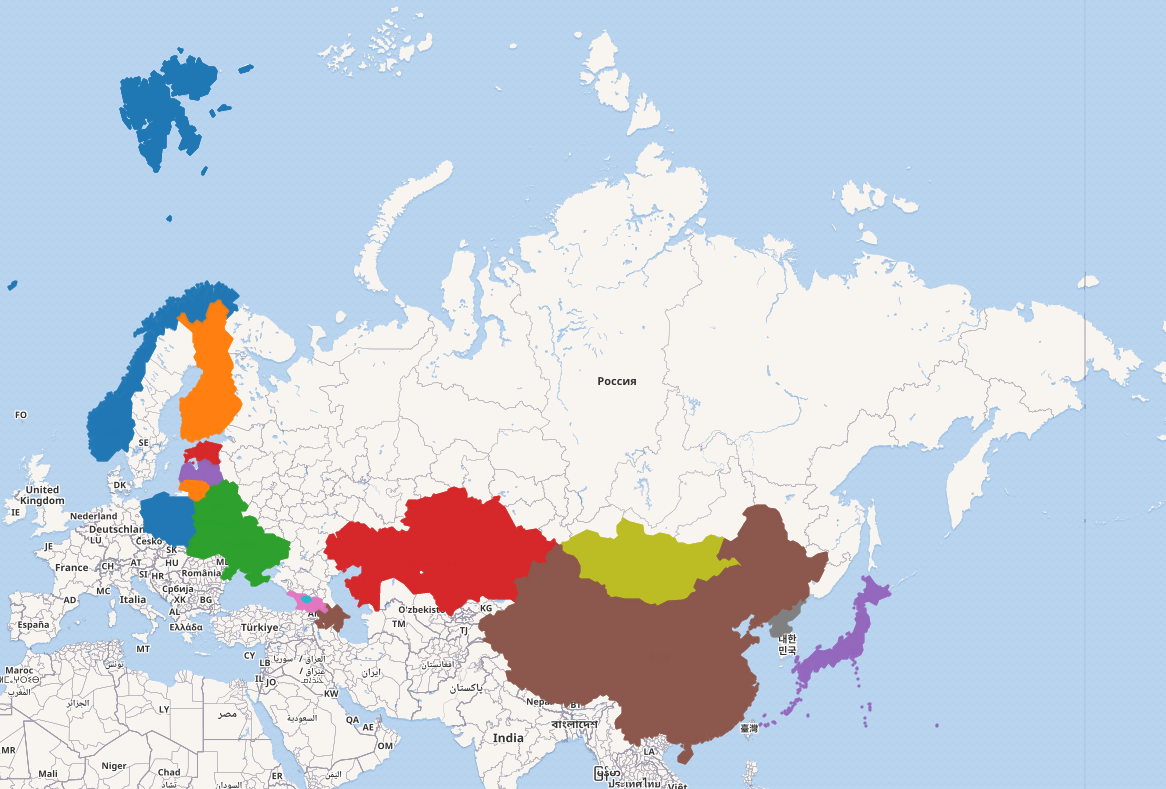
\includegraphics[width=\linewidth]{./chapter/country/Map_of_neighboring_countries_of_Russia_en.png}}%
	}
	\caption{Map of neighboring countries of Russia, 2021.}%
	\label{fig:neighboring_countries_ru}%
\end{figure*}
%%%%%%%%%%%%%%%%%%%%%%%%%%%%%%%%%%%%%%%%%%%%%%%%%%%%%%%
\section{Exercises}

\begin{enumerate}
\item Build a list of country flags and mottos. Not all countries have mottos.
\item Mark the capitals of modern countries on the map.
\item In each part of the world, calculate the top five countries with the highest population density.
\item Build a bar graph showing the distribution of the number of countries by government. Evaluate whether this distribution is a ``heavy tail''\protect\footnotemark.
\footnotetext {In probability theory, heavy-tailed distributions are probability distributions whose tails are not exponentially bounded: that is, they have heavier tails than the exponential distribution. An example of a ``heavy tail'' is shown in Fig. \ref{fig: city_relation_S_N} (dependence of the number of cities on the number of twin cities) on page \pageref{lst: city_relation_S_N}.}
\item Print the list of countries sorted by the number of neighbors. Which countries have the most and least neighbors, what is the average number of neighbors? Is there a correlation between this indicator and any other country dimension?
\end{enumerate}
